\newcommand{\boxcomment}[1]{\textcolor{blue}{\emph{\dotfill(#1)}}}

\section{Evaluation Measures in the Appendix}

In the appendix, in multiple cases, we also report regret, the forgone utility from an actual model prediction in comparison to the oracle choice. 
Intuitively, regret measures how many interactions the model handled poorly throughout the experiment. 
In our experiments, regret is the accumulated number of incorrect examples throughout learning. 
Regret gives a single number that considers both the final performance and how fast the model reached it. 
A good system would reach high performance as fast as possible, making fewer mistakes overall (i.e., would have a low regret).

In some cases, we also report train accuracy as the running mean accuracy over the most recent 256 episodes. 


\section{Additional Method Analysis}\label{appendix:icrl}


    

    

\subsection{\naiveshort and \naiveplus Hyperparameters}

We study the effect of the model sampling temperature $T$ on both \naiveshort and \naiveplus (\autoref{fig:naive:temperature_sensitivity}). For \naiveshort (\autoref{fig:naive:temperature_sensitivity:naive}), we observe that varying $T$ does not significantly affect performance, and all values lead to relatively poor results. 
In contrast, \naiveplus is highly sensitive to $T$ (\autoref{fig:naive:temperature_sensitivity:naive_plus}): while higher temperatures can sometimes reach stronger performance, they also introduce substantial instability. 
Low temperatures are more stable but plateau at lower levels of accuracy. Overall, we find that $T=2.0$ achieves both good performance and stability. 
We adopt this value for all subsequent \naiveplusshort experiments, including the ablations reported in \autoref{fig:results_ablations}.

A related concern involves zero-shot performance (i.e., performance at time step 0). Because we use $T=1.0$ for \expshort (and \naiveshort) and $T=2.0$ for \naiveplusshort, it is unclear whether to measure zero-shot performance with $T=1.0$ or $T=2.0$. To ensure fairness, in all experiments combining \naiveplusshort and \expshort, we report the higher of these two zero-shot accuracies as our baseline. In particular, in many instances, because of this choice, the difference between final and initial performance exceeds the difference between final and zero-shot performance.


\begin{figure*}[b!]
    \centering
    
    \begin{subfigure}[b]{0.99\textwidth}
        \centering
        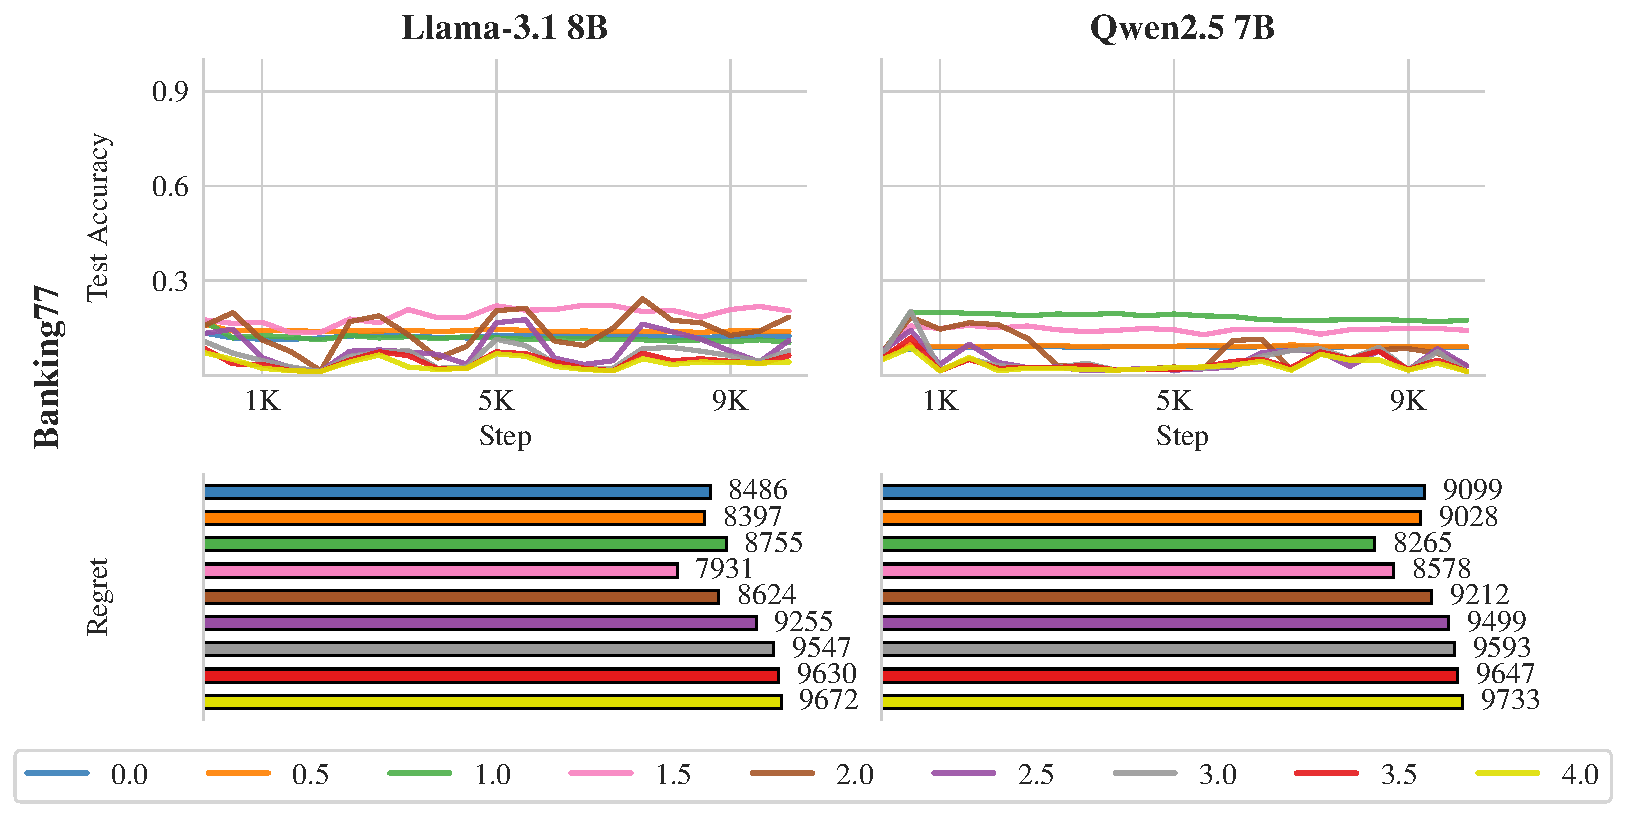
\includegraphics[width=1.0\textwidth]{figures/main_results/temp_sensitivity_random_biased_end.pdf}
        \caption{\textbf{Temperature Sensitivity Analysis for \naiveshort.}}
        \label{fig:naive:temperature_sensitivity:naive}
    \end{subfigure}
    \vspace{2em}

    \begin{subfigure}[b]{0.99\textwidth}
        \centering
        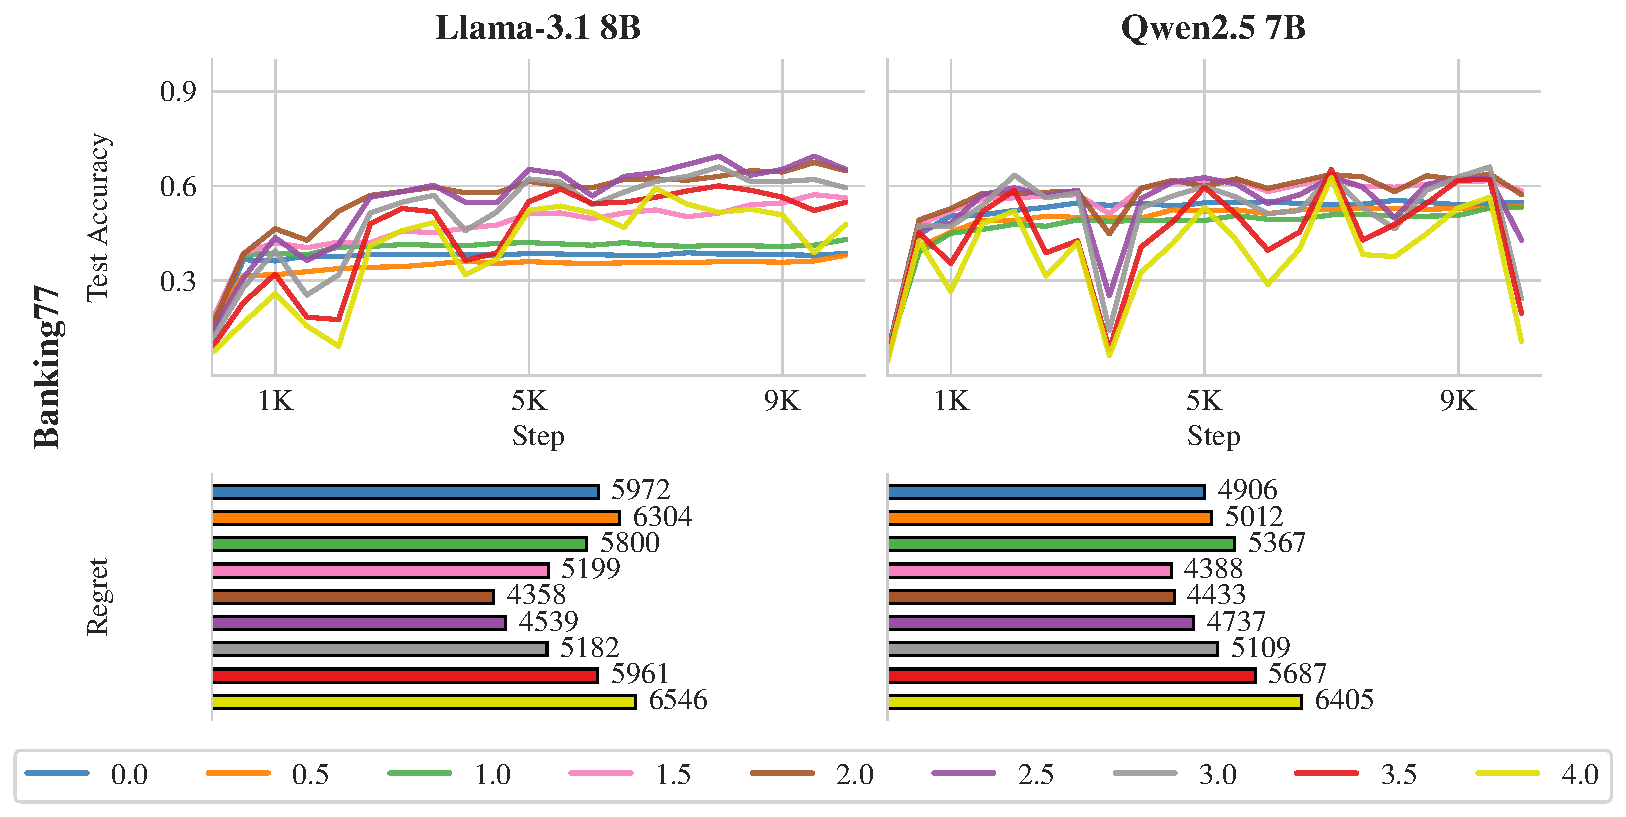
\includegraphics[width=1.0\textwidth]{figures/main_results/temp_sensitivity_random_biased_end_only_positive.pdf}
        \caption{\textbf{Temperature Sensitivity Analysis for \naiveplusshort.}}
        \label{fig:naive:temperature_sensitivity:naive_plus}
    \end{subfigure}
    \vspace{2em}
    
    \caption{\textbf{Temperature Sensitivity Analysis for \naiveshort and \naiveplusshort.} We plot the performance of each approach across different sampling temperatures $T$. (a) For \naiveshort, varying $T$ has little impact, and all temperature settings result in relatively poor performance. (b) \naiveplusshort exhibits significant variability: higher $T$ values can lead to strong performance but are less stable, whereas lower $T$ values yield more stable results but with lower peak accuracy. We choose $T=2.0$ for \naiveplusshort to achieve both strong performance and stability.}
    \label{fig:naive:temperature_sensitivity}
\end{figure*}



\subsection{\explorative}

\subsubsection{Downsampling Strategies}

In our formulation of \explorative, we downsample too large contexts by randomly removing selected episodes until they fit the model context. However, we design three strategies in total to downsample the context if we reach the limit of the LLM context window: (a) \textit{unbiased} (the default strategy): randomly remove episodes from $\context^{(t)}$ until it fits the context window; (b) \textit{start-biased}: use the longest possible prefix of episodes from $\context^{(t)}$ such that it fits the LLM context size; and (c) \textit{end-biased}: use the longest possible suffix. Unbiased corresponds to the approach used in the main paper. 

In practice, we never saturate the LLM context window when using \explorative with $\keepprob=0.1$ because our context windows are more than 100k. 
We conduct experiments to evaluate the above strategiesby limiting the context window of \llama to 4k or 8k tokens. 
Generally, we observe that \textit{start-biased} strategy outperforms \textit{unbiased}, which in turn performs better than \textit{end-biased}, in all cases, although by only small margins. Given these results, we focus on \textit{unbiased} as the most straightforward approach.
\autoref{fig:combined_results_explor_context_strategies} shows the results of this analysis for \banking and \clinic. 

\subsubsection{Hyperparameter Tuning and Sensitivity}

Stochasticity in context generation is one of the key components that contribute to both \expshort performance. It is controlled by setting $\keepprob$. \autoref{fig:results_p_keep} shows the sensitivity of \expshort to different values of $\keepprob$. Without stochasticity ($\keepprob = 1.0$), ICRL struggles on both models—particularly on \phillm—while setting $\keepprob$ too low retains too few examples in the context and hurts performance. Setting $\keepprob = 0.1$ strikes a good balance, yielding strong results while keeping the context short (and therefore faster to run). We fix $\keepprob$ to 0.1 for all subsequent \expshort experiments.

We do not optimize the sampling temperature $T$ for \expshort in this work and simply fix it to a standard value of 1.0. It is possible that performance could improve further with a more optimal temperature selection. We leave this investigation to future work.

\begin{figure*}[t!]
    \centering
    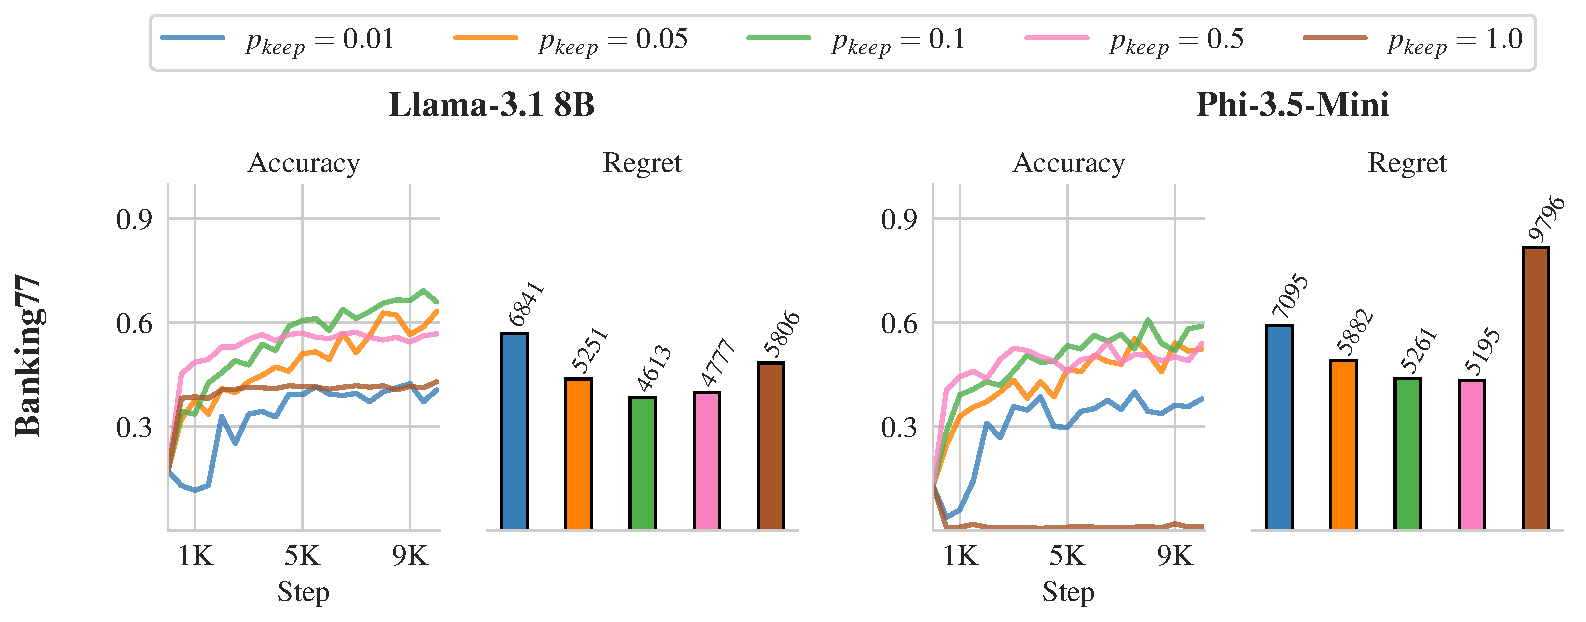
\includegraphics[width=0.9\textwidth]{figures/p_keep_search/p_keep_search_results.pdf}
    \caption{\textbf{Sensitivity to $\keepprob$ in \explorative}. We compare performance with different values of $\keepprob$. Intermediate values learn better for both \llama and \phillm.}
    \label{fig:results_p_keep}
\end{figure*}





\begin{figure}[t!]
    \centering
    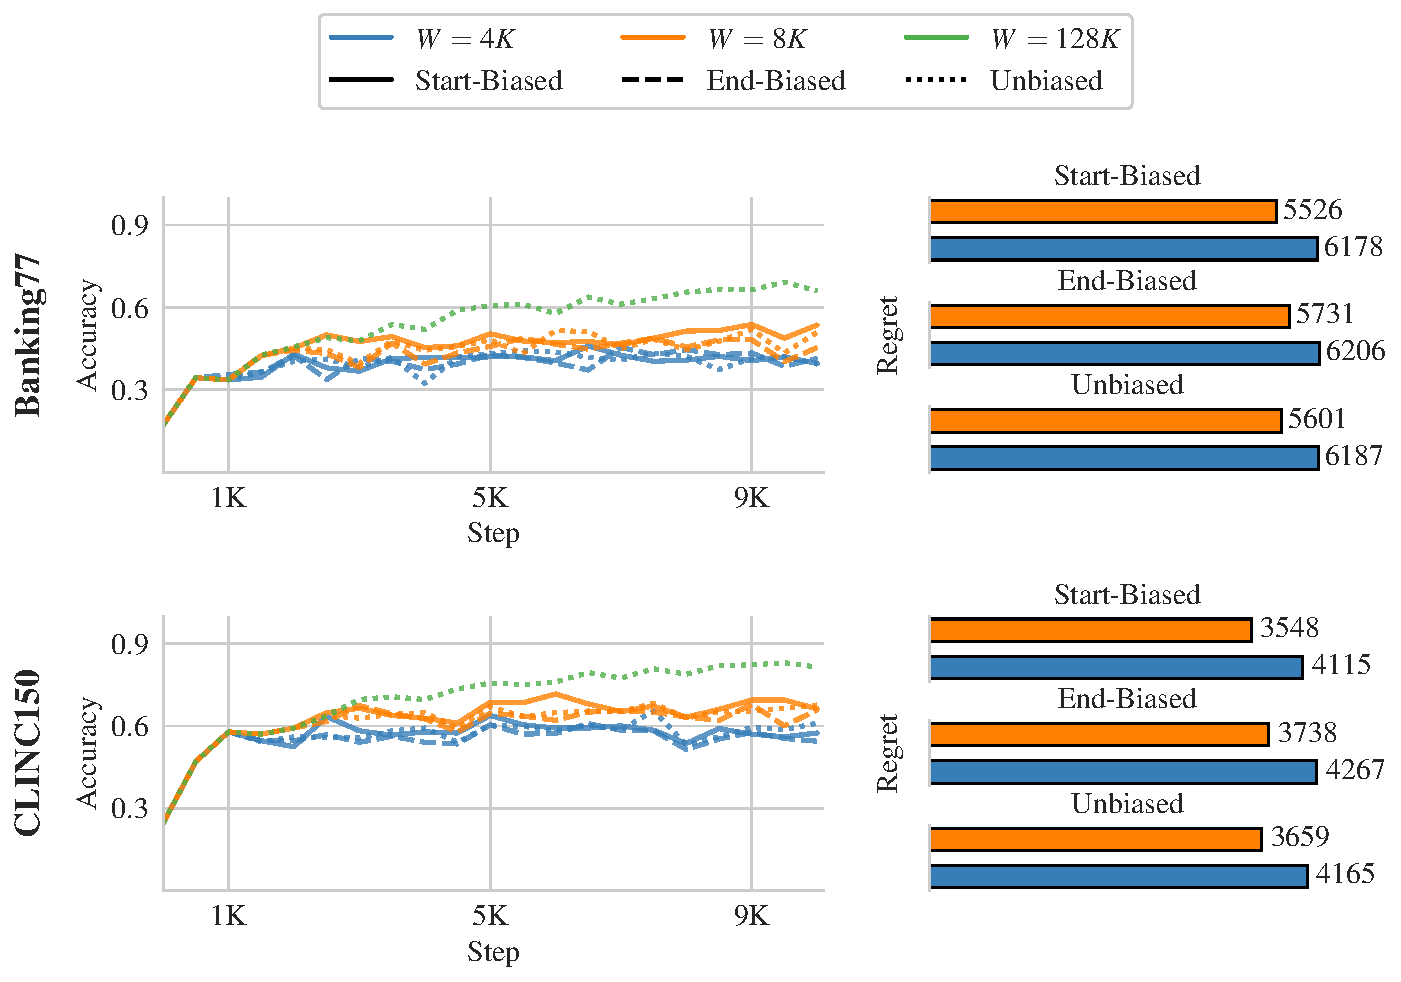
\includegraphics[width=0.8\textwidth]{figures/context_length_strategy_comparison/context_length_and_strategy_comparison.pdf}
    \caption{\textbf{Varying Maximum Context in \llama for \banking and \clinic.} Comparison of test accuracy and regret of \llama under varying context lengths and subsampling strategies for both \banking and \clinic datasets. Longer contexts generally enhance performance, with subtle differences observed between subsampling strategies. The difference between the strategies is negligible.}
    \label{fig:combined_results_explor_context_strategies}
\end{figure}







\begin{algorithm}[!t]
    \footnotesize
    \caption{\approximate}\label{alg:approximate_icrl}
    \begin{algorithmic}[1]
        \REQUIRE
        \STATEX Everything from \autorefalg{alg:explorative_icrl}
        \STATEX $\storagesize$: Number of contexts to maintain
        \STATEX
        \STATE Init empty contexts $\mathcal{C} \gets \{[\,]^{(1)},\dots,[\,]^{(\storagesize)}\}$ \label{ln:aicrl:init_contexts}%
        \FOR{$t=1,2,3,\dots$}
            \STATE Sample context uniformally $\context \sim \uniform \left( \mathcal{C} \right)$ \label{ln:aicrl:sample_context}
            \STATE Observe input $\example^{(t)} \sim \datadist$ \label{ln:aicrl:input}
            \STATE Sample prediction $\hat{\prediction}^{(t)} \sim \policy( \cdot \vert \context, \example^{(t)})$
            \STATE Observe reward $\reward^{(t)} \sim \rewardfunc(\example^{(t)}, \hat{\prediction}^{(t)})$  \label{ln:aicrl:reward} %
            \IF{$r > 0$} \label{ln:aicrl:testreward}
                \FOR{$k = 1$ to $\storagesize$}\label{ln:aicrl:itercontexts}
                    \STATE $b \sim \text{Bernoulli}(\keepprob)$
                    \IF{$b = 1$}
                        \STATE Add episode to cached context \par \hspace{4em} $\contextstore[k] \mathrel{+}= (\example^{(t)}, \hat{\prediction}^{(t)}, \reward^{(t)})$ \label{ln:aicrl:updatecontext} %
                    \ENDIF
                \ENDFOR
            \ENDIF
        \ENDFOR
    \end{algorithmic}
\end{algorithm}


\subsection{\approximate}\label{sec:icrl:approximate}

\subsubsection{\explorative Computational Costs}


An important technical difference between the \naiveshort and \naiveplusshort approaches and \expshort is that, until the context window is not saturated, \naiveshort approaches can potentially re-use past computations from caching. This is not possible in \expshort, because each episode requires the construction of a fresh context $\context^{(t)}$. The probability of encountering the same context twice, or even the same prefix, is exceptionally low even after a few episodes. 
This means that the context has to be computed from scratch for each input.\footnote{In low-memory setups, this does not lead to noticeable slowdowns (as efficient caching would not be possible), and \expshort can be much faster given that each context contains only $\keepprob$\% of the episodes that \naiveplusshort would use. In our setup, we empirically find this to be the case and \expshort is significantly faster in practice.}



\subsubsection{Method}
We propose an approximation of \explorative that balances between computational cost and learning effectiveness. 
Similar to both \naiveplusshort and \expshort, the approximate version also excludes episodes with negative reward and, like \expshort, focuses on exploration by stochasticity in the context. 

\autorefalg{alg:approximate_icrl} describes \approximate. 
The core idea behind the approximation is to persistently store a limited number of contexts, so we can simply gradually expand them with new episodes, rather than always create and compute new contexts. 
We maintain $\storagesize$ contexts $\contextstore$, which all start empty (line~\ref{ln:aicrl:init_contexts}). 
At each time step $t$, we sample a context $\context$ from the $\storagesize$ contexts (line~\ref{ln:aicrl:sample_context}), and use it for episode $t$ (lines \ref{ln:aicrl:input}--\ref{ln:aicrl:reward}. 
If the reward $\reward^{(t)}>0$, we use the episode to expand all contexts stochastically. 
For each context in $\contextstore$, we expand it with the $t$-th episode with a probability of $\keepprob$ (lines \ref{ln:aicrl:itercontexts}--\ref{ln:aicrl:updatecontext}). 

\appshort introduces stochasticity in two places: sampling the context to use for each episode and the expansion of the stored contexts. 
In \autorefalg{alg:approximate_icrl}, we use \emph{uniform} sampling to choose the context (line~\ref{ln:aicrl:sample_context}). 
This is a uniform approximation of the probability of a context, which can also be easily computed \emph{exactly} using the probabilities of the episodes it contains and $\keepprob$. 
In practice, we find the exact computation to work poorly, because contexts that are assigned more episodes or have low probability episodes quickly receive very low probability, and are not used. 
\autoref{fig:results_approximate_parameters:sampling_strategies} shows this experimental analysis.
We use uniform sampling throughout our experiments. 


The level of approximation the algorithm provides depends on the resources available. For example, one can allocate each context to a compute unit, so a machine with eight compute units (e.g., GPUs) will support $\storagesize=8$. 
\appshort is a strict approximation of \expshort in the sense that coupling the exact context sampling strategy with $\storagesize \to \infty$ gives \expshort. 
However, the approximation is limited in handling contexts that extend beyond the LLM window length. Overcoming this while maintaining the efficiency of the approximation is an important direction for future work. 


\subsubsection{Results}

We test \appshort on \llama and \phillm only, and show the results in \autoref{fig:main_results_with_phi_and_approximate}. If not specified, we choose $\storagesize = 8$ for \appshort.

\begin{figure*}[t!]
    \centering

    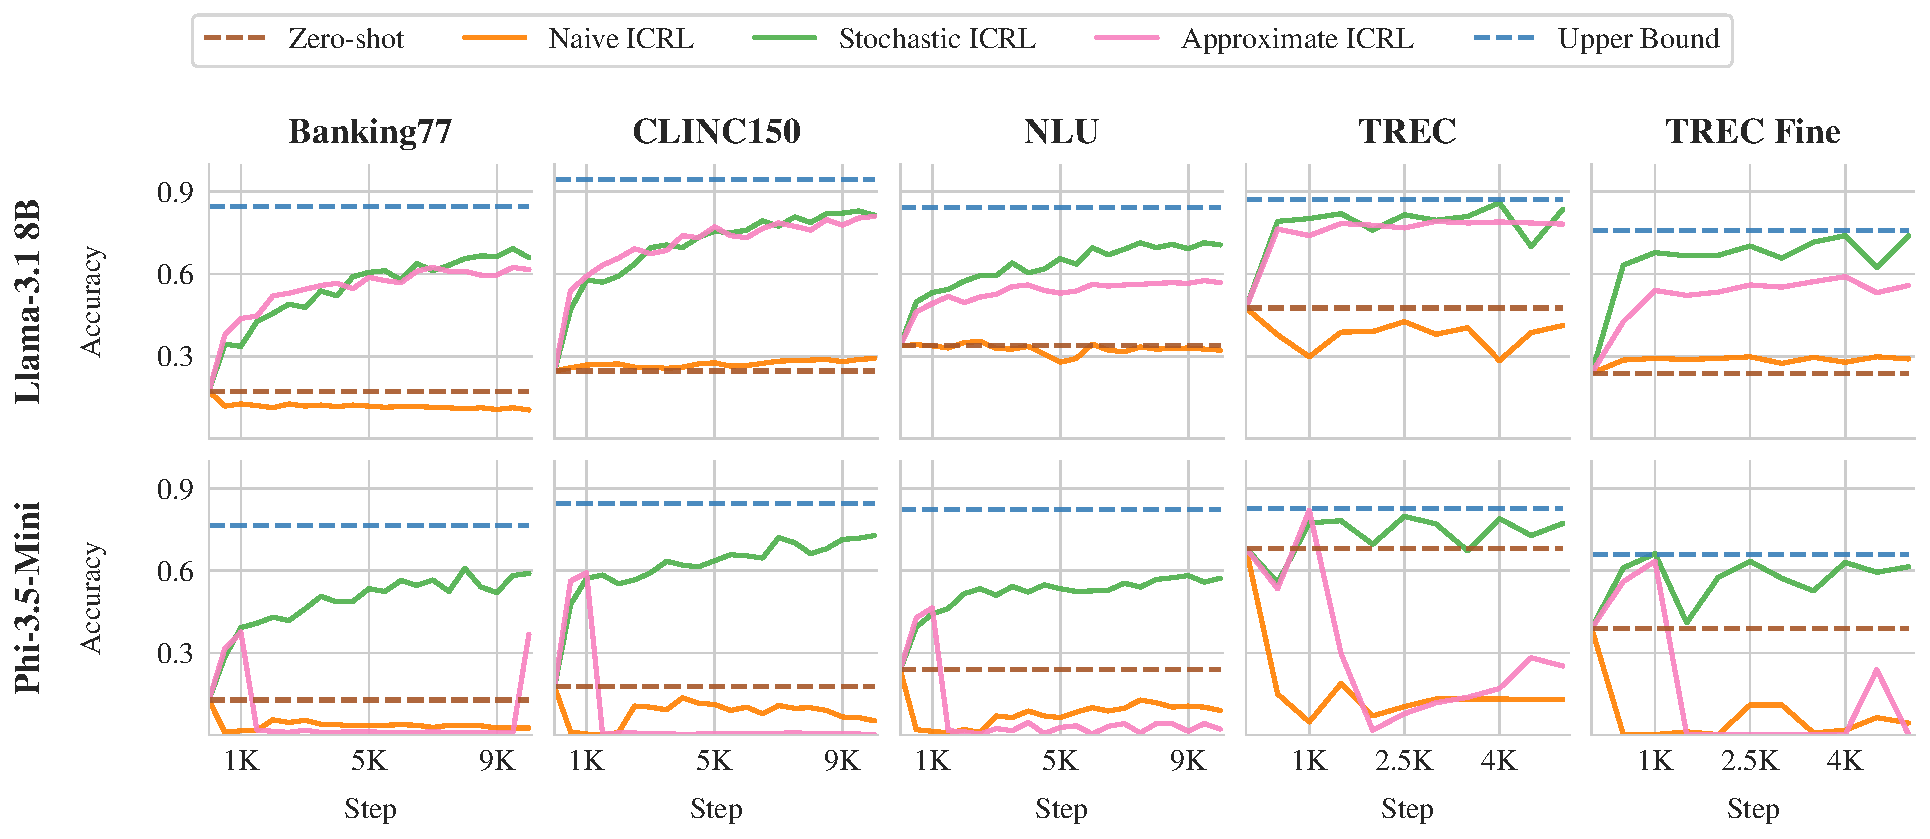
\includegraphics[width=1.0\textwidth]{figures/main_results/main_results_phi_and_approximate.pdf}
    \caption{\textbf{Performance of ICRL}. \expshort and \appshort held-out test results for both \llama and \phillm and all semantic-labels tasks.}
    \label{fig:main_results_with_phi_and_approximate}
\end{figure*}


\paragraph{\appshort is an Effective Alternative to \expshort}

In \autoref{fig:main_results_with_phi_and_approximate}, \appshort performs almost as well as \explorative when using \llama, across all tasks. 
The results are very different with \phillm: despite early learning, \appshort deteriorates quickly. 
This stems from one of the contexts being biased towards one label and therefore predicting only this label. Eventually, the bias towards the label spreads to other contexts, leading to the collapse in performance we observe. 
It is empirically possible to recover, as we see in \banking later in the experiment, but the chance of it happening seems low. 
The success of \llama and failure of \phillm with $\storagesize = 8$ show that different LLMs have different sensitivity to the approximation. 
\autoref{fig:results_approximate_parameters:beam_size} shows that that with a higher number of contexts $\storagesize > 32$ \phillm is able to effectively learn, indicating \phillm needs a higher computational budget. 
On the other hand, \llama is robust to the approximation, with most values performing similarly to \expshort, except with the lowest values of $\storagesize$.

\paragraph{\appshort Reduces Compute Needs.}

We measure the reduction of tokens processed in \appshort compared to \expshort throughout full ICRL runs. 
We approximate this measure by computing at each step the number of tokens required for a forward call and subtracting the number of tokens of the sequence with the longest common prefix processed in a previous step, as it would be possible to use the KV cache for all the tokens in the common prefix (assuming infinite memory). We find that \expshort processes two orders of magnitude more tokens than \appshort. \autoreftab{tab:token_usage_comparison} provides numerical results for this analysis.

\begin{figure*}[t]
\centering

\begin{subfigure}[b]{\textwidth}
\centering
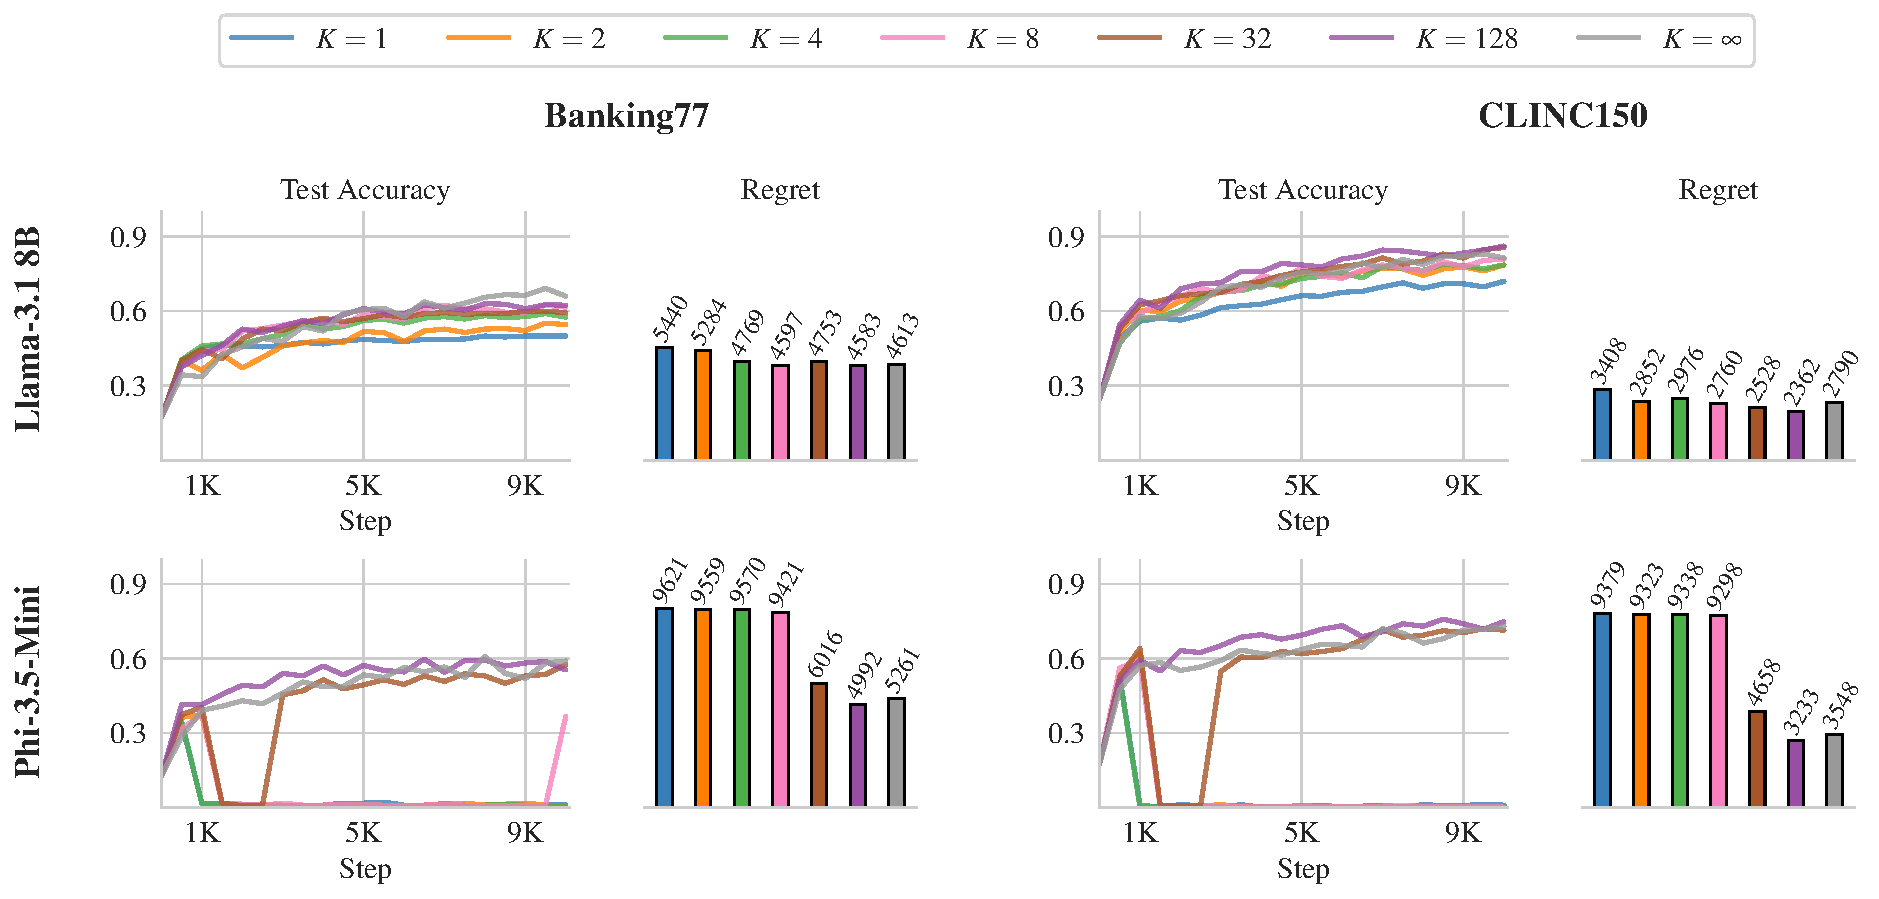
\includegraphics[width=0.99\textwidth]{figures/approximate_beam_sizes/approximate_beam_sizes_results.pdf}
\caption{\textbf{Effect of the number of contexts}.}
\label{fig:results_approximate_parameters:beam_size}
\end{subfigure}
\hfill


\begin{subfigure}[b]{\textwidth}
\centering
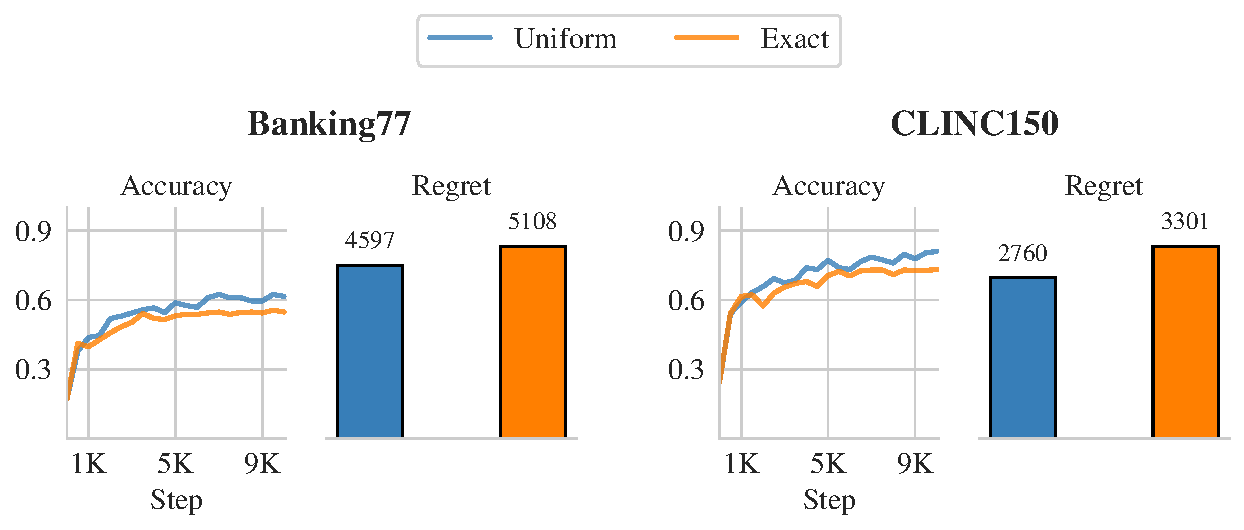
\includegraphics[width=0.65\textwidth]{figures/approximate_sampling_methods/approximate_context_sampling_method_comparison.pdf}
\caption{\textbf{Effect of the context sampling strategies}.}
\label{fig:results_approximate_parameters:sampling_strategies}
\end{subfigure}


\caption{\textbf{Comparison of \appshort parameters}. (a) Effect of the number of contexts $\storagesize$. We report test accuracy for \llama and \phillm. \phillm proves more sensitive to this approximation. Generation degenerates for low $\storagesize$, while the model can learn for $\storagesize \geq 32$. \llama can learn with all $\storagesize$, although higher values perform better. (b) Comparison of exact and uniform sampling. We report test accuracy at the final step and regret for \llama. Uniform sampling strategy is consistently better.}
\label{fig:results_approximate_parameters}
\end{figure*}




\section{Experimental Setup}\label{sec:appendix:exp_setup} 
We conduct experiments on various type of GPUs: 40GB A100, 80GB A100, 80GB H100, 48GB A6000. For experiments with 70B and 32B models, we use 4 80GB A100/H100 or 8 48GB A6000. For experiments with 14B models, we use 2 80GB A100/H100. For experiments with 7B or smaller models, we use 1 80GB A100/H100 or 2 48GB A6000 / 40GB A100. For efficient inference, we use \textit{vllm}~\citep{kwon2023efficientmemorymanagementlarge}.

\subsection{Prompt Design}\label{appendix:exp_setup:prompt}

We report prompt examples from ICL (\autoref{fig:prompt_example_icl}) and ICRL (\autoref{fig:prompt_example_icrl}) experiments. We show the prompts for \llama as an example. In all cases, we show the prompts with two in-context examples.




\begin{figure}[ht]
    \centering
    \begin{tcolorbox}[width=0.9\textwidth, fonttitle=\bfseries, title={Prompt example for ICL in \llama}]
\begin{Verbatim}[breaklines=true, breakanywhere=true]
<|begin_of_text|><|start_header_id|>system<|end_header_id|>\n\nCutting Knowledge Date: December 2023\nToday Date: 26 Jul 2024\n\nYou are an useful assistant. Answer the following questions.<|eot_id|><|start_header_id|>user<|end_header_id|>\n\nQuery: Tell me about the card PIN?<|eot_id|><|start_header_id|>assistant<|end_header_id|>\n\nIntent: get physical card<|eot_id|><|start_header_id|>user<|end_header_id|>\n\nQuery: Is there a daily auto top-up limit?<|eot_id|><|start_header_id|>assistant<|end_header_id|>\n\nIntent: automatic top up<|eot_id|><|start_header_id|>user<|end_header_id|>\n\nQuery: I got a message saying I made a withdrawal from the bank machine, but I did not.<|eot_id|><|start_header_id|>assistant<|end_header_id|>\n\nIntent:
\end{Verbatim}
    \end{tcolorbox}
    \caption{\textbf{An example of prompt of ICL for \llama.}}
    \label{fig:prompt_example_icl}
\end{figure}




\begin{figure}[ht]
    \centering
    \begin{tcolorbox}[width=0.9\textwidth, fonttitle=\bfseries, title={Prompt example for ICRL in \llama}]
\begin{Verbatim}[breaklines=true, breakanywhere=true]
<|begin_of_text|><|start_header_id|>system<|end_header_id|>\n\nCutting Knowledge Date: December 2023\nToday Date: 26 Jul 2024\n\nYou are an useful assistant. Answer the following questions. Feedback will indicate if you answered correctly. You must answer correctly, using previous feedback to make better predictions.<|eot_id|><|start_header_id|>user<|end_header_id|>\n\nQuery: It declined my transfer.<|eot_id|><|start_header_id|>assistant<|end_header_id|>\n\nIntent: declined transfer<|eot_id|><|start_header_id|>user<|end_header_id|>\n\n'declined transfer' is the correct answer! Good job!\n\nQuery: Am I allowed to change my PIN anywhere?<|eot_id|><|start_header_id|>assistant<|end_header_id|>\n\nIntent: verify top up<|eot_id|><|start_header_id|>user<|end_header_id|>\n\nThe answer 'verify top up' is wrong! You can do better!\n\nQuery: If I'm getting my identity verified, what all do I need?<|eot_id|><|start_header_id|>assistant<|end_header_id|>\n\nIntent:
\end{Verbatim}
    \end{tcolorbox}
    \caption{\textbf{An example of prompt of ICRL for \llama.}}
    \label{fig:prompt_example_icrl}
\end{figure}










\subsection{Context Windows and Episode Capacity}\label{appendix:exp_setup:data}

For each task and model combination, we conservatively estimate the maximum number of examples that could fit within the context window. This is done by including all observed examples in descending order of token count in the prompt, assuming the model consistently responds with the longest label and that the formatted reward message is at its maximum length. We perform this calculation using the maximum context window for all models. Additionally, for \llama, we repeat the process with context windows of 4{,}096 and 8{,}192 tokens specifically for the \banking and \clinic tasks. 
\autoreftab{tab:appendix_max_examples_per_task_model} reports episode capacity.

\begin{table}[!t]
\caption{\textbf{Maximum number of episodes supported by model and task, given a specific context window}. We compute the maximum number of episodes supported by the context window of \llama, \phillm, \qwen, and \gemini across all tasks, including 4k and 8k tokens for \llama, with \banking and \clinic only.}
\centering
\footnotesize
\begin{tabular}{lcccccc}
\toprule
& \textbf{\phillm} & \multicolumn{3}{c}{\textbf{\llama}} & \textbf{\qwen} & \textbf{\gemini} \\
\cmidrule(lr){2-2} \cmidrule(lr){3-5} \cmidrule(lr){6-7}
\textbf{Task} & 128k tokens & 4k tokens & 8k tokens & 128k tokens & 128k tokens & 1M tokens \\

\midrule
\textbf{\banking}   & 1538  & 34 & 74 & 1673 & 1672 & - \\
\textbf{\clinic}    & 2241  & 60 & 126 & 2384 & 2184 & - \\
\textbf{\nlu}       & 2397  & -  & -   & 2425 & 2424 & - \\
\textbf{\trec}      & 2848  & -  & -   & 2919 & 2896 & - \\
\textbf{\trecfine}  & 2584  & -  & -   & 2776 & 2755 & - \\
\midrule
\textbf{Abs. \banking}   & -  & - & - & 1924 & 1788 & 13007 \\
\textbf{Abs. \clinic}    & -  & - & - & 2485 & 2270 & 19501 \\
\textbf{Abs. \nlu}       & -  & - & - & 2475 & 2285 & 24603 \\
\textbf{Abs. \trec}      & -  & - & - & 2529 & 2308 & 5953 \\
\textbf{Abs. \trecfine}  & -  & - & - & 2531 & 2308 & 5953 \\
\midrule[\heavyrulewidth]
\end{tabular}
\label{tab:appendix_max_examples_per_task_model}
\end{table}



\subsection{Datasets}\label{sec:appendix:datasets}

We use 5 classification tasks (and the corresponding abstract-label variants) in our experiments:
\begin{itemize}
    \item \banking~(77 labels; \citet{Casanueva2020}). It involves 77 labels and aims to detect the intent of user queries in an economic context. For example, one label could be ``\textit{balance not updated after cheque or cash deposit}".
    \item \clinic~(150 labels; \citet{larson-etal-2019-evaluation}. It includes 150 labels, also focusing on intent classification. An example label is ``\textit{calendar update}". While the original dataset was designed to detect out-of-scope queries, we concentrate solely on classifying the 150 defined intents, excluding out-of-scope queries from our analysis.
    \item \nlu~(68 labels; \citet{Liu2021}). This dataset includes queries grouped in 68 unique categories for human-robot interaction in home domain (for example, one label is ``\textit{audio volume mute}".  
    \item \trec and \trecfine~(respectively 6 and 50 labels; \citet{li-roth-2002-learning, hovy-etal-2001-toward}). Both are question classification dataset where the goal is to classify the type of question. Each example contains both a fine label (that we use in \trecfine), as ``\textit{entity vehicle}", and a coarse one (used in \trec), as ``\textit{entity}". \trecfine includes 50 categories, while \trec groups them in only 6 categories.
\end{itemize}

All of these datasets are  challenging because of the big number of different labels, and the sometimes subtle differences between labels. Moreover, in our setting we do not provide any information about the list of potential labels (except for the ``With Exemplars" abstract-label experiments), challenging the model to either follow previously discovered labels or try to find new, more suitable ones (i.e., exploitation vs exploration -- \citet{sutton2018reinforcement}).


\section{Additional Results}\label{sec:appendix:results}

\begin{table}[t]
\caption{%
  \textbf{Detailed Figures for \autoref{fig:main_results}.}
  We report three key figures for each dataset and method: initial (zero-shot) accuracy, final (post-ICRL) accuracy, and regret (total mistakes). (a) contains the results for \llama, (b) for \qwen.
}
\scriptsize
\centering
\subfloat[\textbf{\llama}]{
\begin{tabular}{l ccc ccc ccc c}
\toprule
& \multicolumn{3}{c}{\textbf{\naiveshort}} 
& \multicolumn{3}{c}{\textbf{\naiveplusshort}} 
& \multicolumn{3}{c}{\textbf{\expshort}} 
& \textbf{Upper Bound} \\
\cmidrule(lr){2-4}
\cmidrule(lr){5-7}
\cmidrule(lr){8-10}
\cmidrule(lr){11-11}
\textbf{Dataset} & 0-step & Final & Reg. & 0-step & Final & Reg. & 0-step & Final & Reg. & Acc. \\
& Acc. & Acc. &  & Acc. & Acc. &  & Acc. & Acc. &  &  \\
\midrule
\textbf{\banking}  & 0.172 & 0.104 & 8755 & 0.152 & 0.648 & 4358 & 0.172 & 0.660 & 4613 & 0.846 \\
\textbf{\clinic}   & 0.246 & 0.292 & 7126 & 0.092 & 0.836 & 2280 & 0.246 & 0.814 & 2790 & 0.944 \\
\textbf{\nlu}        & 0.338 & 0.322 & 6868 & 0.286 & 0.578 & 4486 & 0.338 & 0.706 & 3545 & 0.844 \\
\textbf{\trec}       & 0.476 & 0.412 & 3692 & 0.326 & 0.744 & 2235 & 0.476 & 0.836 & 1183 & 0.872 \\
\textbf{\trecfine}  & 0.238 & 0.29  & 4390 & 0.070 & 0.610 & 2585 & 0.238 & 0.740 & 2183 & 0.760 \\
\midrule[\heavyrulewidth]
\end{tabular}
\label{tab:main_results:llama}
}

\vspace{1em} %

\subfloat[\textbf{\qwen}]{
\begin{tabular}{l ccc ccc ccc c}
\toprule
& \multicolumn{3}{c}{\textbf{\naiveshort}} 
& \multicolumn{3}{c}{\textbf{\naiveplusshort}} 
& \multicolumn{3}{c}{\textbf{\expshort}} 
& \textbf{Upper Bound} \\
\cmidrule(lr){2-4}
\cmidrule(lr){5-7}
\cmidrule(lr){8-10}
\cmidrule(lr){11-11}
\textbf{Dataset} & 0-step & Final & Reg. & 0-step & Final & Reg. & 0-step & Final & Reg. & Acc. \\
& Acc. & Acc. &  & Acc. & Acc. &  & Acc. & Acc. &  &  \\
\midrule
\textbf{\banking}  & 0.064 & 0.174 & 8265 & 0.070 & 0.572 & 4433 & 0.062 & 0.722 & 4274 & 0.862 \\
\textbf{\clinic}   & 0.154 & 0.108 & 8691 & 0.138 & 0.802 & 2378 & 0.154 & 0.838 & 2913 & 0.960 \\
\textbf{\nlu}        & 0.216 & 0.230 & 7369 & 0.248 & 0.788 & 2967 & 0.208 & 0.748 & 3235 & 0.874 \\
\textbf{\trec}       & 0.430 & 0.292 & 3883 & 0.372 & 0.664 & 2477 & 0.440 & 0.806 & 1181 & 0.880 \\
\textbf{\trecfine}  & 0.146 & 0.014 & 4734 & 0.122 & 0.536 & 3337 & 0.144 & 0.704 & 1920 & 0.812 \\
\midrule[\heavyrulewidth]
\end{tabular}
\label{tab:main_results:qwen}
}
\label{tab:main_results}
\end{table}


\begin{table}[t]
\caption{%
\textbf{Detailed Metrics for \autoref{fig:results_ablations}.}
We report three key metrics for each dataset and method: initial (zero-shot) accuracy, final (post-ICRL) accuracy, and regret (total mistakes). (a) shows results for \banking, (b) for \clinic.
}
\centering
\scriptsize

\vspace{1em} %

\subfloat[\textbf{\banking}]{
\begin{tabular}{l ccc ccc}
\toprule
& \multicolumn{3}{c}{\textbf{\naiveshort}}
& \multicolumn{3}{c}{\textbf{\expshort}}\\
\cmidrule(lr){2-4}
\cmidrule(lr){5-7}
\textbf{Reward}
& 0-step & Final & Reg.
& 0-step & Final & Reg.\\
& Acc. & Acc. &
& Acc. & Acc. &
\\
\midrule
\textbf{None} 
  & 0.156 & 0.034 & 9426
  & 0.172 & 0.308 & 7132\\
\textbf{Only neg.} 
  & 0.152 & 0.060 & 9331
  & 0.172 & 0.214 & 7814\\
\textbf{Only pos.} 
  & 0.152 & 0.648 & 4358
  & 0.172 & 0.660 & 4613\\
\textbf{Both pos. and neg.} 
  & 0.156 & 0.184 & 8624
  & 0.172 & 0.458 & 5943\\
\textbf{Noisy pos. and neg.} 
  & 0.156 & 0.174 & 8713
  & 0.172 & 0.394 & 6256\\
\textbf{Inv. pos. and neg.} 
  & 0.152 & 0.098 & 9234
  & 0.172 & 0.282 & 7047\\
\midrule[\heavyrulewidth]
\end{tabular}
\label{tab:results_ablations:banking}
}

\vspace{1em} %

\subfloat[\textbf{\clinic}]{
\begin{tabular}{l ccc ccc}
\toprule
& \multicolumn{3}{c}{\textbf{\naiveshort}}
& \multicolumn{3}{c}{\textbf{\expshort}}\\
\cmidrule(lr){2-4}
\cmidrule(lr){5-7}
\textbf{Reward}
& 0-step & Final & Reg.
& 0-step & Final & Reg.\\
& Acc. & Acc. &
& Acc. & Acc. &
\\
\midrule
\textbf{None} 
  & 0.092 & 0.056 & 9214
  & 0.246 & 0.388 & 6555\\
\textbf{Only neg.} 
  & 0.092 & 0.082 & 9010
  & 0.246 & 0.208 & 7496\\
\textbf{Only pos.} 
  & 0.092 & 0.836 & 2280
  & 0.246 & 0.814 & 2790\\
\textbf{Both pos. and neg.} 
  & 0.092 & 0.170 & 8280
  & 0.246 & 0.582 & 4688\\
\textbf{Noisy pos. and neg.} 
  & 0.092 & 0.146 & 8454
  & 0.246 & 0.586 & 4810\\
\textbf{Inv. pos. and neg.} 
  & 0.092 & 0.098 & 8995
  & 0.246 & 0.448 & 5865\\
\midrule[\heavyrulewidth]
\end{tabular}
\label{tab:results_ablations:clinic}
}
\label{tab:results_ablations}
\end{table}







\begin{table}[t]
\caption{%
  \textbf{Detailed Figures for \autoref{fig:abstract_tasks}.}
  We report three key figures for each dataset and method: initial (zero-shot) accuracy, final (post-ICRL) accuracy, and regret (total mistakes).
}
\label{tab:abstract_tasks}
\scriptsize
\centering

\subfloat[\llama\ Accuracies]{
  \begin{tabular}{l cc  cc  cc  cc  cc}
  \toprule
    & \multicolumn{2}{c}{\textbf{Abs. \banking}} 
    & \multicolumn{2}{c}{\textbf{Abs. \clinic}} 
    & \multicolumn{2}{c}{\textbf{Abs. \nlu}} 
    & \multicolumn{2}{c}{\textbf{Abs. \trec}} 
    & \multicolumn{2}{c}{\textbf{Abs. \trecfine}} \\
  \cmidrule(lr){2-3}\cmidrule(lr){4-5}\cmidrule(lr){6-7}\cmidrule(lr){8-9}\cmidrule(lr){10-11}
  \textbf{Method} 
  & 0-step & Final 
  & 0-step & Final 
  & 0-step & Final 
  & 0-step & Final 
  & 0-step & Final \\
  \midrule
  \textbf{\naiveshort}               & 0.020 & 0.018 & 0.002 & 0.000 & 0.010 & 0.028 & 0.030 & 0.086 & 0.034 & 0.030 \\
  \textbf{\naiveplusshort (w/o Ex.)}  & 0.020 & 0.454 & 0.008 & 0.276 & 0.010 & 0.476 & 0.118 & 0.790 & 0.080 & 0.144 \\
  \textbf{\naiveplusshort (w/ Ex.)}   & 0.024 & 0.178 & 0.000 & 0.590 & 0.056 & 0.656 & 0.238 & 0.792 & 0.006 & 0.196 \\
  \textbf{\expshort (w/o Ex.)}        & 0.018 & 0.350 & 0.002 & 0.162 & 0.010 & 0.428 & 0.030 & 0.838 & 0.034 & 0.258 \\
  \textbf{\expshort (w/ Ex.)}         & 0.030 & 0.584 & 0.006 & 0.650 & 0.162 & 0.722 & 0.238 & 0.840 & 0.008 & 0.036 \\
  \midrule
  \textbf{Up. Bound Acc.}            &       & 0.780 &       & 0.886 &       & 0.750 &       & 0.886 &       & 0.612 \\
  \bottomrule
  \end{tabular}
}
\quad
\subfloat[\llama\ Regrets]{
  \begin{tabular}{l c  c  c  c  c}
  \toprule
    & \textbf{Abs. \banking} 
    & \textbf{Abs. \clinic} 
    & \textbf{Abs. \nlu} 
    & \textbf{Abs. \trec} 
    & \textbf{Abs. \trecfine} \\
  \cmidrule(lr){2-6}
  \textbf{Method} 
  & Reg. 
  & Reg. 
  & Reg. 
  & Reg. 
  & Reg. \\
  \midrule
  \textbf{\naiveshort}               & 9909  & 9928  & 9674  & 4032  & 4828  \\
  \textbf{\naiveplusshort (w/o Ex.)}  & 7164  & 8507  & 6789  & 2046  & 4597  \\
  \textbf{\naiveplusshort (w/ Ex.)}   & 4704  & 5727  & 4166  & 2214  & 4153  \\
  \textbf{\expshort (w/o Ex.)}        & 8280  & 9437  & 7288  & 2244  & 4767  \\
  \textbf{\expshort (w/ Ex.)}         & 4380  & 6276  & 3725  & 2424  & 4773  \\
  \bottomrule
  \end{tabular}
}

\vspace{1em}

\subfloat[\qwen\ Accuracies]{
  \begin{tabular}{l cc  cc  cc  cc  cc}
  \toprule
    & \multicolumn{2}{c}{\textbf{Abs. \banking}} 
    & \multicolumn{2}{c}{\textbf{Abs. \clinic}} 
    & \multicolumn{2}{c}{\textbf{Abs. \nlu}} 
    & \multicolumn{2}{c}{\textbf{Abs. \trec}} 
    & \multicolumn{2}{c}{\textbf{Abs. \trecfine}} \\
  \cmidrule(lr){2-3}\cmidrule(lr){4-5}\cmidrule(lr){6-7}\cmidrule(lr){8-9}\cmidrule(lr){10-11}
  \textbf{Method} 
  & 0-step & Final 
  & 0-step & Final 
  & 0-step & Final 
  & 0-step & Final 
  & 0-step & Final \\
  \midrule
  \textbf{\naiveshort}               & 0.016 & 0.002 & 0.012 & 0.014 & 0.010 & 0.014 & 0.124 & 0.130 & 0.010 & 0.024 \\
  \textbf{\naiveplusshort (w/o Ex.)}  & 0.014 & 0.442 & 0.008 & 0.204 & 0.014 & 0.622 & 0.136 & 0.526 & 0.010 & 0.146 \\
  \textbf{\naiveplusshort (w/ Ex.)}   & 0.248 & 0.626 & 0.048 & 0.602 & 0.162 & 0.656 & 0.158 & 0.776 & 0.004 & 0.526 \\
  \textbf{\expshort (w/o Ex.)}        & 0.016 & 0.208 & 0.012 & 0.134 & 0.010 & 0.564 & 0.124 & 0.886 & 0.010 & 0.532 \\
  \textbf{\expshort (w/ Ex.)}         & 0.316 & 0.680 & 0.080 & 0.712 & 0.182 & 0.706 & 0.200 & 0.890 & 0.002 & 0.462 \\
  \midrule
  \textbf{Up. Bound Acc.}            &       & 0.844 &       & 0.902 &       & 0.822 &       & 0.892 &       & 0.574 \\
  \bottomrule
  \end{tabular}
}
\quad
\subfloat[\qwen\ Regrets]{
  \begin{tabular}{l c  c  c  c  c}
  \toprule
    & \textbf{Abs. \banking} 
    & \textbf{Abs. \clinic} 
    & \textbf{Abs. \nlu} 
    & \textbf{Abs. \trec} 
    & \textbf{Abs. \trecfine} \\
  \cmidrule(lr){2-6}
  \textbf{Method} 
  & Reg. 
  & Reg. 
  & Reg. 
  & Reg. 
  & Reg. \\
  \midrule
  \textbf{\naiveshort}               & 9877  & 9892  & 9731  & 3876  & 4810 \\
  \textbf{\naiveplusshort (w/o Ex.)}  & 7391  & 8824  & 6479  & 3304  & 3713 \\
  \textbf{\naiveplusshort (w/ Ex.)}   & 4618  & 4481  & 3818  & 1564  & 3044 \\
  \textbf{\expshort (w/o Ex.)}        & 8653  & 9449  & 6128  & 1591  & 3868 \\
  \textbf{\expshort (w/ Ex.)}         & 4353  & 4385  & 3882  & 1520  & 4440 \\
  \bottomrule
  \end{tabular}
}

\vspace{1em}

\subfloat[\gemini\ Accuracies]{
  \begin{tabular}{l cc  cc  cc  cc  cc}
  \toprule
    & \multicolumn{2}{c}{\textbf{Abs. \banking}} 
    & \multicolumn{2}{c}{\textbf{Abs. \clinic}} 
    & \multicolumn{2}{c}{\textbf{Abs. \nlu}} 
    & \multicolumn{2}{c}{\textbf{Abs. \trec}} 
    & \multicolumn{2}{c}{\textbf{Abs. \trecfine}} \\
  \cmidrule(lr){2-3}\cmidrule(lr){4-5}\cmidrule(lr){6-7}\cmidrule(lr){8-9}\cmidrule(lr){10-11}
  \textbf{Method} 
  & 0-step & Final 
  & 0-step & Final 
  & 0-step & Final 
  & 0-step & Final 
  & 0-step & Final \\
  \midrule
  \textbf{\naiveshort}               & 0.018 & 0.000 & 0.008 & 0.010 & 0.048 & 0.004 & 0.076 & 0.012 & 0.002 & 0.018 \\
  \textbf{\naiveplusshort (w/o Ex.)}  & 0.014 & 0.174 & 0.002 & 0.144 & 0.044 & 0.218 & 0.104 & 0.900 & 0.006 & 0.130 \\
  \textbf{\naiveplusshort (w/ Ex.)}   & 0.430 & 0.778 & 0.356 & 0.818 & 0.474 & 0.774 & 0.480 & 0.896 & 0.134 & 0.682 \\
  \textbf{\expshort (w/o Ex.)}        & 0.014 & 0.214 & 0.008 & 0.060 & 0.050 & 0.290 & 0.072 & 0.876 & 0.002 & 0.060 \\
  \textbf{\expshort (w/ Ex.)}         & 0.440 & 0.792 & 0.434 & 0.858 & 0.480 & 0.794 & 0.494 & 0.872 & 0.138 & 0.636 \\
  \midrule
  \textbf{Up. Bound Acc.}            &       & 0.902 &       & 0.964 &       & 0.890 &       & 0.946 &       & 0.860 \\
  \bottomrule
  \end{tabular}
}
\quad
\subfloat[\gemini\ Regrets]{
  \begin{tabular}{l c  c  c  c  c}
  \toprule
    & \textbf{Abs. \banking} 
    & \textbf{Abs. \clinic} 
    & \textbf{Abs. \nlu} 
    & \textbf{Abs. \trec} 
    & \textbf{Abs. \trecfine} \\
  \cmidrule(lr){2-6}
  \textbf{Method} 
  & Reg. 
  & Reg. 
  & Reg. 
  & Reg. 
  & Reg. \\
  \midrule
  \textbf{\naiveshort}               & 9996  & 9929  & 9938  & 4841  & 4915 \\
  \textbf{\naiveplusshort (w/o Ex.)}  & 8858  & 9264  & 7978  & 1308  & 3998 \\
  \textbf{\naiveplusshort (w/ Ex.)}   & 2776  & 1711  & 2582  & 1127  & 2448 \\
  \textbf{\expshort (w/o Ex.)}        & 8625  & 9710  & 8281  & 1505  & 4920 \\
  \textbf{\expshort (w/ Ex.)}         & 3292  & 1984  & 2560  & 1439  & 3420 \\
  \bottomrule
  \end{tabular}
}

\end{table}




\begin{table*}[t]
\caption{%
\textbf{Detailed Metrics for \autoref{fig:scaling_compact}.}
We report three key metrics for each dataset and method: initial (zero-shot) accuracy, final (post-ICRL) accuracy, and regret (total mistakes).
(a)--(g) show results for different sizes of Qwen2.5.
}
\centering
\scriptsize

\begin{subtable}{.48\textwidth}
\caption{\textbf{Qwen2.5 500M}}
\centering
\begin{tabular}{l ccc ccc}
\toprule
 & \multicolumn{3}{c}{\textbf{\naiveplusshort}}
 & \multicolumn{3}{c}{\textbf{\expshort}}\\
\cmidrule(lr){2-4}
\cmidrule(lr){5-7}
\textbf{Dataset}
& 0-step & Final & Reg.
& 0-step & Final & Reg.\\
\midrule
\textbf{\banking}   & 0.082 & 0.284 & 7351 & 0.146 & 0.364 & 6874 \\
\textbf{\clinic}    & 0.062 & 0.404 & 5959 & 0.118 & 0.552 & 5157 \\
\textbf{\nlu}       & 0.088 & 0.358 & 6746 & 0.146 & 0.544 & 6162 \\
\textbf{\trec}      & 0.290 & 0.382 & 2260 & 0.318 & 0.514 & 2182 \\
\textbf{\trecfine}  & 0.032 & 0.154 & 3955 & 0.034 & 0.308 & 3961 \\
\midrule[\heavyrulewidth]
\end{tabular}
\end{subtable}
\hfill
\begin{subtable}{.48\textwidth}
\caption{\textbf{Qwen2.5 1.5B}}
\centering
\begin{tabular}{l ccc ccc}
\toprule
 & \multicolumn{3}{c}{\textbf{\naiveplusshort}}
 & \multicolumn{3}{c}{\textbf{\expshort}}\\
\cmidrule(lr){2-4}
\cmidrule(lr){5-7}
\textbf{Dataset}
& 0-step & Final & Reg.
& 0-step & Final & Reg.\\
\midrule
\textbf{\banking}   & 0.074 & 0.258 & 6069 & 0.092 & 0.524 & 5824 \\
\textbf{\clinic}    & 0.066 & 0.482 & 4660 & 0.182 & 0.684 & 3945 \\
\textbf{\nlu}       & 0.242 & 0.302 & 5084 & 0.288 & 0.636 & 4619 \\
\textbf{\trec}      & 0.274 & 0.302 & 2150 & 0.362 & 0.754 & 1835 \\
\textbf{\trecfine}  & 0.042 & 0.538 & 2979 & 0.074 & 0.680 & 2681 \\
\midrule[\heavyrulewidth]
\end{tabular}
\end{subtable}

\vspace{1em}

\begin{subtable}{.48\textwidth}
\caption{\textbf{Qwen2.5 3B}}
\centering
\begin{tabular}{l ccc ccc}
\toprule
 & \multicolumn{3}{c}{\textbf{\naiveplusshort}}
 & \multicolumn{3}{c}{\textbf{\expshort}}\\
\cmidrule(lr){2-4}
\cmidrule(lr){5-7}
\textbf{Dataset}
& 0-step & Final & Reg.
& 0-step & Final & Reg.\\
\midrule
\textbf{\banking}   & 0.082 & 0.532 & 4959 & 0.094 & 0.614 & 4852 \\
\textbf{\clinic}    & 0.156 & 0.778 & 2370 & 0.148 & 0.812 & 2936 \\
\textbf{\nlu}       & 0.270 & 0.734 & 3355 & 0.266 & 0.772 & 2666 \\
\textbf{\trec}      & 0.428 & 0.744 & 2482 & 0.506 & 0.730 & 1246 \\
\textbf{\trecfine}  & 0.098 & 0.520 & 3439 & 0.214 & 0.620 & 2131 \\
\midrule[\heavyrulewidth]
\end{tabular}
\end{subtable}
\hfill
\begin{subtable}{.48\textwidth}
\caption{\textbf{Qwen2.5 7B}}
\centering
\begin{tabular}{l ccc ccc}
\toprule
 & \multicolumn{3}{c}{\textbf{\naiveplusshort}}
 & \multicolumn{3}{c}{\textbf{\expshort}}\\
\cmidrule(lr){2-4}
\cmidrule(lr){5-7}
\textbf{Dataset}
& 0-step & Final & Reg.
& 0-step & Final & Reg.\\
\midrule
\textbf{\banking}   & 0.070 & 0.572 & 4433 & 0.062 & 0.722 & 4274 \\
\textbf{\clinic}    & 0.138 & 0.802 & 2378 & 0.154 & 0.838 & 2913 \\
\textbf{\nlu}       & 0.248 & 0.788 & 2967 & 0.208 & 0.748 & 3235 \\
\textbf{\trec}      & 0.372 & 0.664 & 2477 & 0.440 & 0.806 & 1181 \\
\textbf{\trecfine}  & 0.122 & 0.536 & 3337 & 0.144 & 0.704 & 1920 \\
\midrule[\heavyrulewidth]
\end{tabular}
\end{subtable}

\vspace{1em}

\begin{subtable}{.48\textwidth}
\caption{\textbf{Qwen2.5 14B}}
\centering
\begin{tabular}{l ccc ccc}
\toprule
 & \multicolumn{3}{c}{\textbf{\naiveplusshort}}
 & \multicolumn{3}{c}{\textbf{\expshort}}\\
\cmidrule(lr){2-4}
\cmidrule(lr){5-7}
\textbf{Dataset}
& 0-step & Final & Reg.
& 0-step & Final & Reg.\\
\midrule
\textbf{\banking}   & 0.126 & 0.506 & 4902 & 0.144 & 0.730 & 4136 \\
\textbf{\clinic}    & 0.192 & 0.800 & 2505 & 0.248 & 0.882 & 2439 \\
\textbf{\nlu}       & 0.348 & 0.574 & 4198 & 0.376 & 0.748 & 3228 \\
\textbf{\trec}      & 0.492 & 0.786 & 2105 & 0.556 & 0.904 & 919  \\
\textbf{\trecfine}  & 0.252 & 0.522 & 2989 & 0.322 & 0.734 & 1869 \\
\midrule[\heavyrulewidth]
\end{tabular}
\end{subtable}
\hfill
\begin{subtable}{.48\textwidth}
\caption{\textbf{Qwen2.5 32B}}
\centering
\begin{tabular}{l ccc ccc}
\toprule
 & \multicolumn{3}{c}{\textbf{\naiveplusshort}}
 & \multicolumn{3}{c}{\textbf{\expshort}}\\
\cmidrule(lr){2-4}
\cmidrule(lr){5-7}
\textbf{Dataset}
& 0-step & Final & Reg.
& 0-step & Final & Reg.\\
\midrule
\textbf{\banking}   & 0.132 & 0.518 & 5015 & 0.144 & 0.778 & 3733 \\
\textbf{\clinic}    & 0.220 & 0.838 & 2164 & 0.280 & 0.884 & 2467 \\
\textbf{\nlu}       & 0.360 & 0.702 & 3588 & 0.380 & 0.768 & 2842 \\
\textbf{\trec}      & 0.590 & 0.622 & 2185 & 0.646 & 0.920 & 770  \\
\textbf{\trecfine}  & 0.264 & 0.516 & 2800 & 0.354 & 0.662 & 1599 \\
\midrule[\heavyrulewidth]
\end{tabular}
\end{subtable}

\vspace{1em}

\begin{subtable}{\textwidth}
\caption{\textbf{Qwen2.5 72B}}
\centering
\begin{tabular}{l ccc ccc}
\toprule
 & \multicolumn{3}{c}{\textbf{\naiveplusshort}}
 & \multicolumn{3}{c}{\textbf{\expshort}}\\
\cmidrule(lr){2-4}
\cmidrule(lr){5-7}
\textbf{Dataset}
& 0-step & Final & Reg.
& 0-step & Final & Reg.\\
\midrule
\textbf{\banking}   & 0.186 & 0.592 & 4404 & 0.212 & 0.794 & 3512 \\
\textbf{\clinic}    & 0.328 & 0.870 & 1714 & 0.360 & 0.906 & 1983 \\
\textbf{\nlu}       & 0.380 & 0.776 & 2520 & 0.438 & 0.794 & 2609 \\
\textbf{\trec}      & 0.392 & 0.656 & 2277 & 0.416 & 0.898 &  782 \\
\textbf{\trecfine}  & 0.100 & 0.706 & 2398 & 0.170 & 0.764 & 1614 \\
\midrule[\heavyrulewidth]
\end{tabular}
\end{subtable}
\label{tab:scaling_compact}
\end{table*}



\begin{table*}[t]
\caption{
\textbf{Detailed Stability Metric \(\rho\) for \autoref{fig:qwen_stability}.}
Each cell contains the stability metric \(\rho\) for the corresponding dataset and method.
(a)--(g) show results for different sizes of Qwen2.5.
}
\centering

\begin{subtable}{.48\textwidth}
\caption{\textbf{Qwen2.5 500M}}
\centering
\begin{tabular}{l c c c}
\toprule
& \textbf{\naiveshort} & \textbf{\naiveplusshort} & \textbf{\expshort} \\
\midrule
\textbf{\banking}  & -0.343 & 0.491 & 0.710 \\
\textbf{\clinic}   & -0.459 & 0.634 & 0.877 \\
\textbf{\nlu}      & -0.025 & 0.045 & 0.868 \\
\textbf{\trec}     & -0.500 & 0.264 & 0.700 \\
\textbf{\trecfine} & -0.202 & 0.164 & 0.724 \\
\midrule[\heavyrulewidth]
\end{tabular}
\end{subtable}
\hfill
\begin{subtable}{.48\textwidth}
\caption{\textbf{Qwen2.5 1.5B}}
\centering
\begin{tabular}{l c c c}
\toprule
& \textbf{\naiveshort} & \textbf{\naiveplusshort} & \textbf{\expshort} \\
\midrule
\textbf{\banking}  & 0.209 & 0.427 & 0.875 \\
\textbf{\clinic}   & -0.369 & 0.278 & 0.949 \\
\textbf{\nlu}      & -0.260 & 0.088 & 0.851 \\
\textbf{\trec}     & -0.500 & 0.064 & 0.501 \\
\textbf{\trecfine} & 0.500 & 0.882 & 0.697 \\
\midrule[\heavyrulewidth]
\end{tabular}
\end{subtable}

\vspace{1em}

\begin{subtable}{.48\textwidth}
\caption{\textbf{Qwen2.5 3B}}
\centering
\begin{tabular}{l c c c}
\toprule
& \textbf{\naiveshort} & \textbf{\naiveplusshort} & \textbf{\expshort} \\
\midrule
\textbf{\banking}  & -0.069 & 0.710 & 0.932 \\
\textbf{\clinic}   & -0.652 & 0.748 & 0.956 \\
\textbf{\nlu}      & -0.857 & 0.711 & 0.925 \\
\textbf{\trec}     & -0.500 & 0.882 & 0.773 \\
\textbf{\trecfine} & 0.500 & 0.210 & 0.564 \\
\midrule[\heavyrulewidth]
\end{tabular}
\end{subtable}
\hfill
\begin{subtable}{.48\textwidth}
\caption{\textbf{Qwen2.5 7B}}
\centering
\begin{tabular}{l c c c}
\toprule
& \textbf{\naiveshort} & \textbf{\naiveplusshort} & \textbf{\expshort} \\
\midrule
\textbf{\banking}  & -0.653 & 0.694 & 0.989 \\
\textbf{\clinic}   & -0.794 & 0.679 & 0.985 \\
\textbf{\nlu}      & -0.570 & 0.661 & 0.963 \\
\textbf{\trec}     & -0.230 & -0.134 & 0.314 \\
\textbf{\trecfine} & -0.674 & 0.784 & 0.487 \\
\midrule[\heavyrulewidth]
\end{tabular}
\end{subtable}

\vspace{1em}

\begin{subtable}{.48\textwidth}
\caption{\textbf{Qwen2.5 14B}}
\centering
\begin{tabular}{l c c c}
\toprule
& \textbf{\naiveshort} & \textbf{\naiveplusshort} & \textbf{\expshort} \\
\midrule
\textbf{\banking}  & 0.394 & 0.548 & 0.964 \\
\textbf{\clinic}   & -0.730 & 0.956 & 0.981 \\
\textbf{\nlu}      & -0.494 & 0.337 & 0.859 \\
\textbf{\trec}     & -0.790 & 0.927 & 0.441 \\
\textbf{\trecfine} & -0.691 & 0.540 & 0.825 \\
\midrule[\heavyrulewidth]
\end{tabular}
\end{subtable}
\hfill
\begin{subtable}{.48\textwidth}
\caption{\textbf{Qwen2.5 32B}}
\centering
\begin{tabular}{l c c c}
\toprule
& \textbf{\naiveshort} & \textbf{\naiveplusshort} & \textbf{\expshort} \\
\midrule
\textbf{\banking}  & -0.218 & 0.684 & 0.972 \\
\textbf{\clinic}   & -0.419 & 0.939 & 0.989 \\
\textbf{\nlu}      & 0.035  & 0.887 & 0.945 \\
\textbf{\trec}     & -0.791 & 0.074 & 0.822 \\
\textbf{\trecfine} & -0.849 & 0.886 & 0.292 \\
\midrule[\heavyrulewidth]
\end{tabular}
\end{subtable}

\vspace{1em}

\begin{subtable}{\textwidth}
\caption{\textbf{Qwen2.5 72B}}
\centering
\begin{tabular}{l c c c}
\toprule
& \textbf{\naiveshort} & \textbf{\naiveplusshort} & \textbf{\expshort} \\
\midrule
\textbf{\banking}  & -0.456 & 0.894 & 0.965 \\
\textbf{\clinic}   & 0.159  & 0.854 & 0.986 \\
\textbf{\nlu}      & -0.633 & 0.461 & 0.910 \\
\textbf{\trec}     & -0.500 & 0.936 & 0.765 \\
\textbf{\trecfine} & -0.500 & 0.970 & 0.600 \\
\midrule[\heavyrulewidth]
\end{tabular}
\end{subtable}
\label{tab:qwen_stability}
\end{table*}






\begin{table}[t!]
\caption{\textbf{Tokens processed in \appshort compared to \expshort throughout full ICRL runs.} \expshort processes two orders of magnitude more tokens than \appshort.}
\centering
\footnotesize
\begin{tabular}{l*{6}{c}}
\toprule
& \multicolumn{3}{c}{\textbf{\phillm}} & \multicolumn{3}{c}{\textbf{\llama}} \\
\cmidrule(lr){2-4} \cmidrule(lr){5-7}
\textbf{Task} & Expl. & Approx. & Ratio & Expl. & Approx. & Ratio \\
\midrule
\textbf{\banking}   & 87,369,607  & 510,786 & 171 & 102,282,989 & 539,367 & 190 \\
\textbf{\clinic}    & 105,545,002 & 398,677 & 265 & 122,455,599 & 440,019 & 278 \\
\textbf{\nlu}       & 89,894,548  & 409,680 & 219 & 114,517,653 & 433,254 & 264 \\
\textbf{\trec}      & 29,306,971  & 212,855 & 138 & 34,509,170  & 229,046 & 151 \\
\textbf{\trecfine}  & 20,658,980  & 222,955 & 93  & 25,522,358  & 234,884 & 109 \\
\midrule[\heavyrulewidth]
\end{tabular}
\label{tab:token_usage_comparison}
\end{table}








\begin{figure}[htbp]
\centering
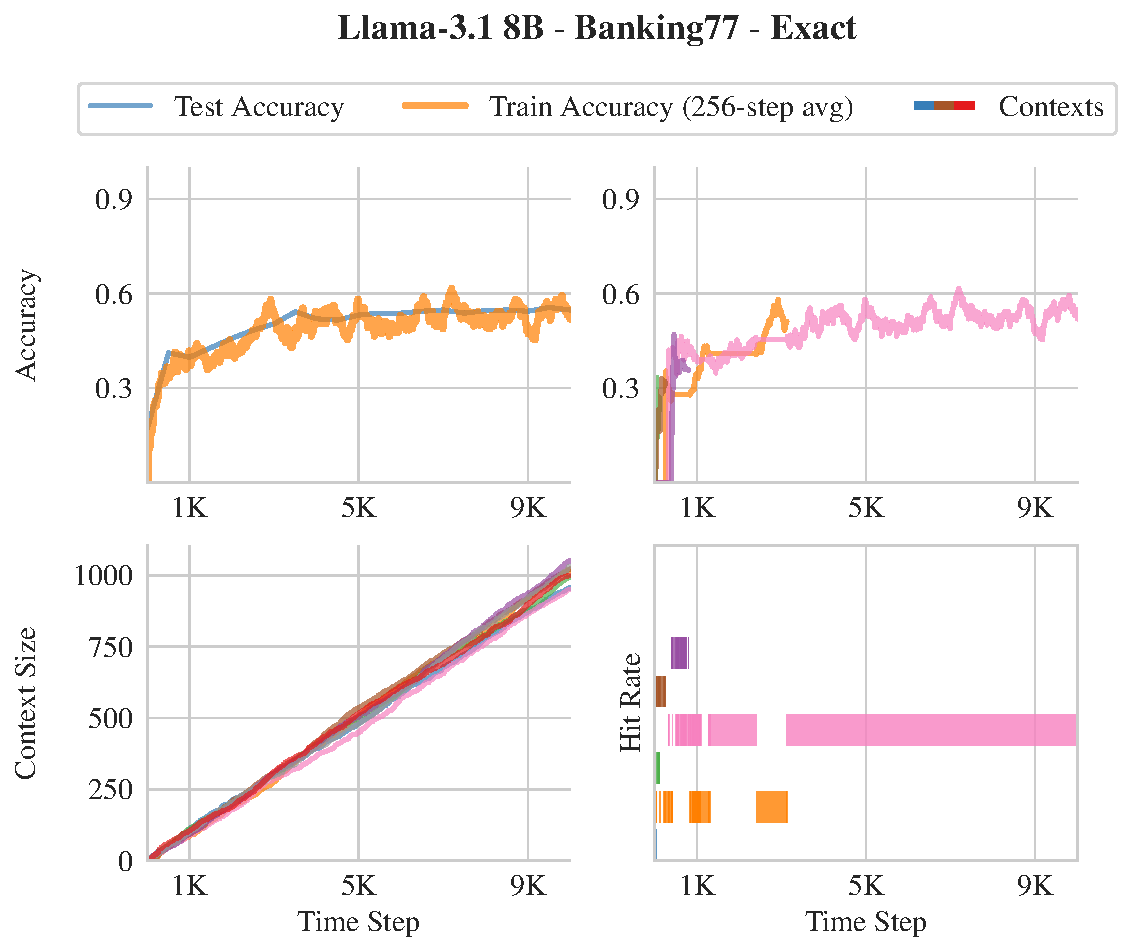
\includegraphics[width=0.6\textwidth]{figures/approximate_detailed_results/meta-llama_Meta-Llama-3.1-8B-Instruct_banking77_exact.pdf}
\caption{\textbf{Detailed visualization of \appshort for \llama, \banking with exact context sampling.} We report test accuracy (top left), a 256-step running average of the training accuracy (bottom left), the training accuracy of each context (top right), and the hit rate of each context (bottom right).}
\end{figure}
\begin{figure}[htbp]
\centering
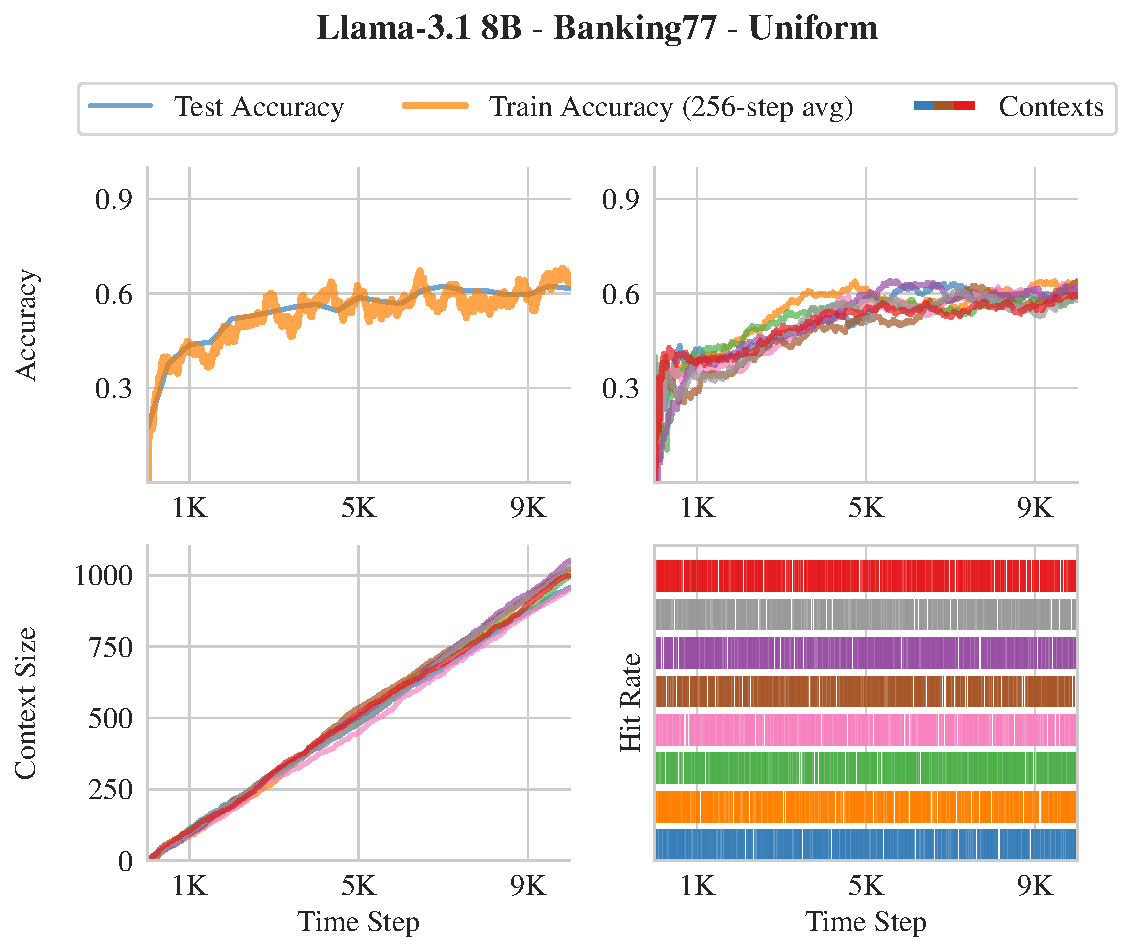
\includegraphics[width=0.6\textwidth]{figures/approximate_detailed_results/meta-llama_Meta-Llama-3.1-8B-Instruct_banking77_uniform.pdf}
\caption{\textbf{Detailed visualization of \appshort for \llama, \banking with uniform context sampling.} We report test accuracy (top left), a 256-step running average of the training accuracy (bottom left), the training accuracy of each context (top right), and the hit rate of each context (bottom right).}
\end{figure}
\begin{figure}[htbp]
\centering
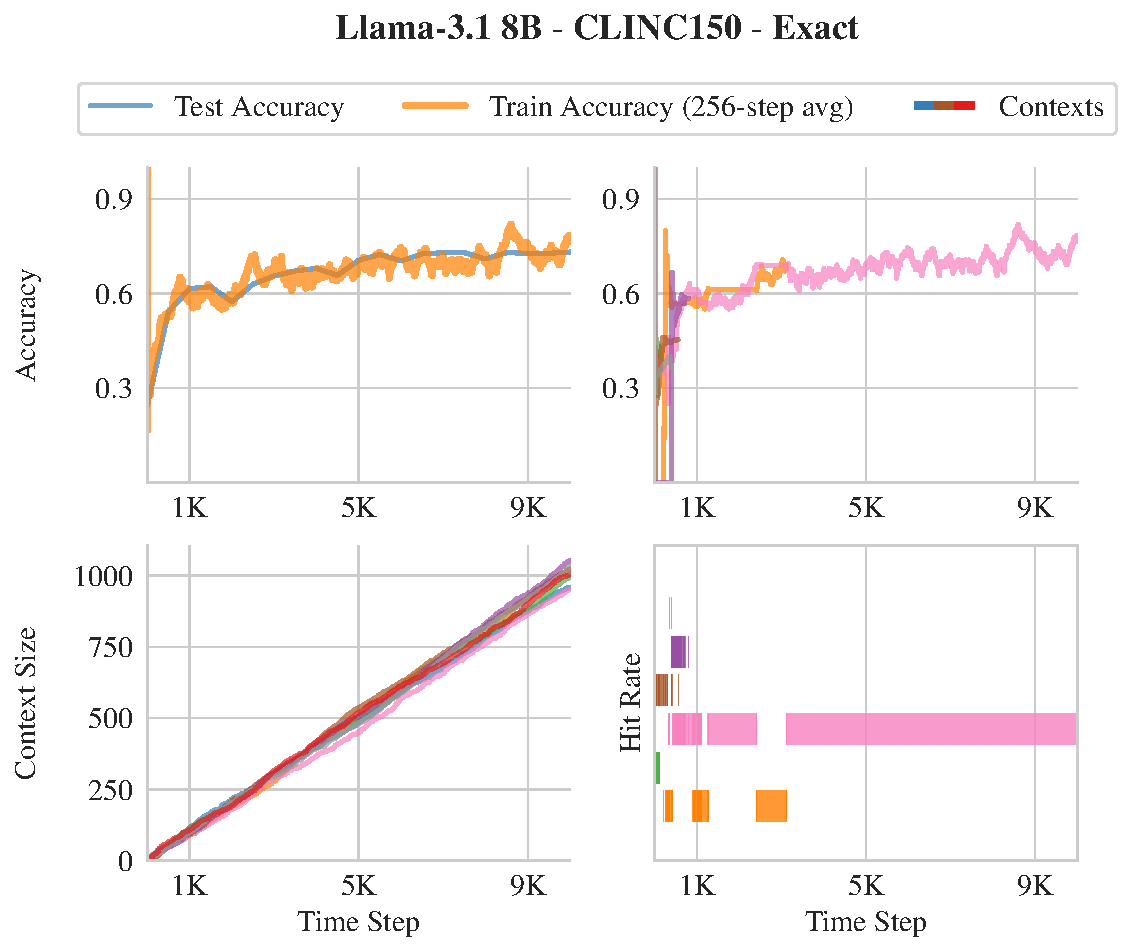
\includegraphics[width=0.6\textwidth]{figures/approximate_detailed_results/meta-llama_Meta-Llama-3.1-8B-Instruct_clinic150_exact.pdf}
\caption{\textbf{Detailed visualization of \appshort for \llama, \clinic with exact context sampling.} We report test accuracy (top left), a 256-step running average of the training accuracy (bottom left), the training accuracy of each context (top right), and the hit rate of each context (bottom right).}
\end{figure}
\begin{figure}[htbp]
\centering
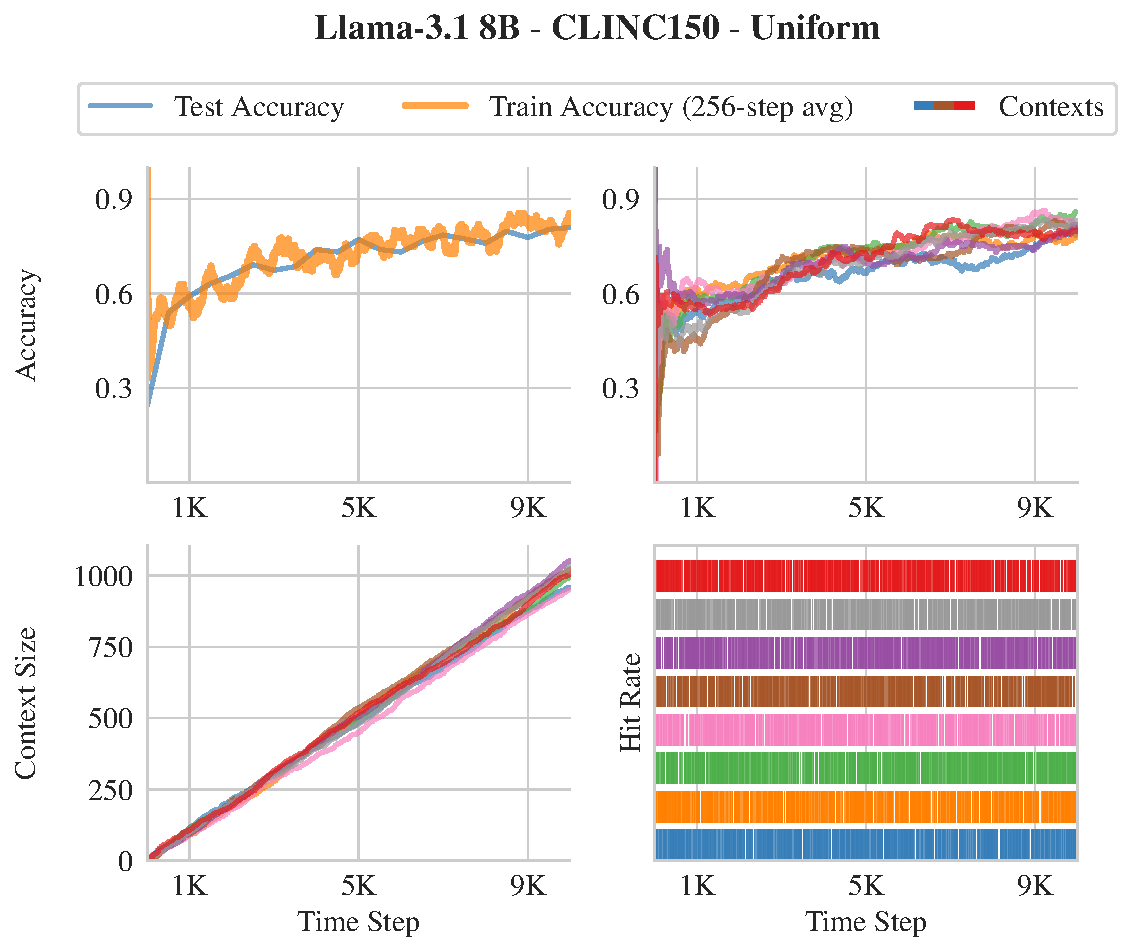
\includegraphics[width=0.6\textwidth]{figures/approximate_detailed_results/meta-llama_Meta-Llama-3.1-8B-Instruct_clinic150_uniform.pdf}
\caption{\textbf{Detailed visualization of \appshort for \llama, \clinic with uniform context sampling.} We report test accuracy (top left), a 256-step running average of the training accuracy (bottom left), the training accuracy of each context (top right), and the hit rate of each context (bottom right).}
\end{figure}
\begin{figure}[htbp]
\centering
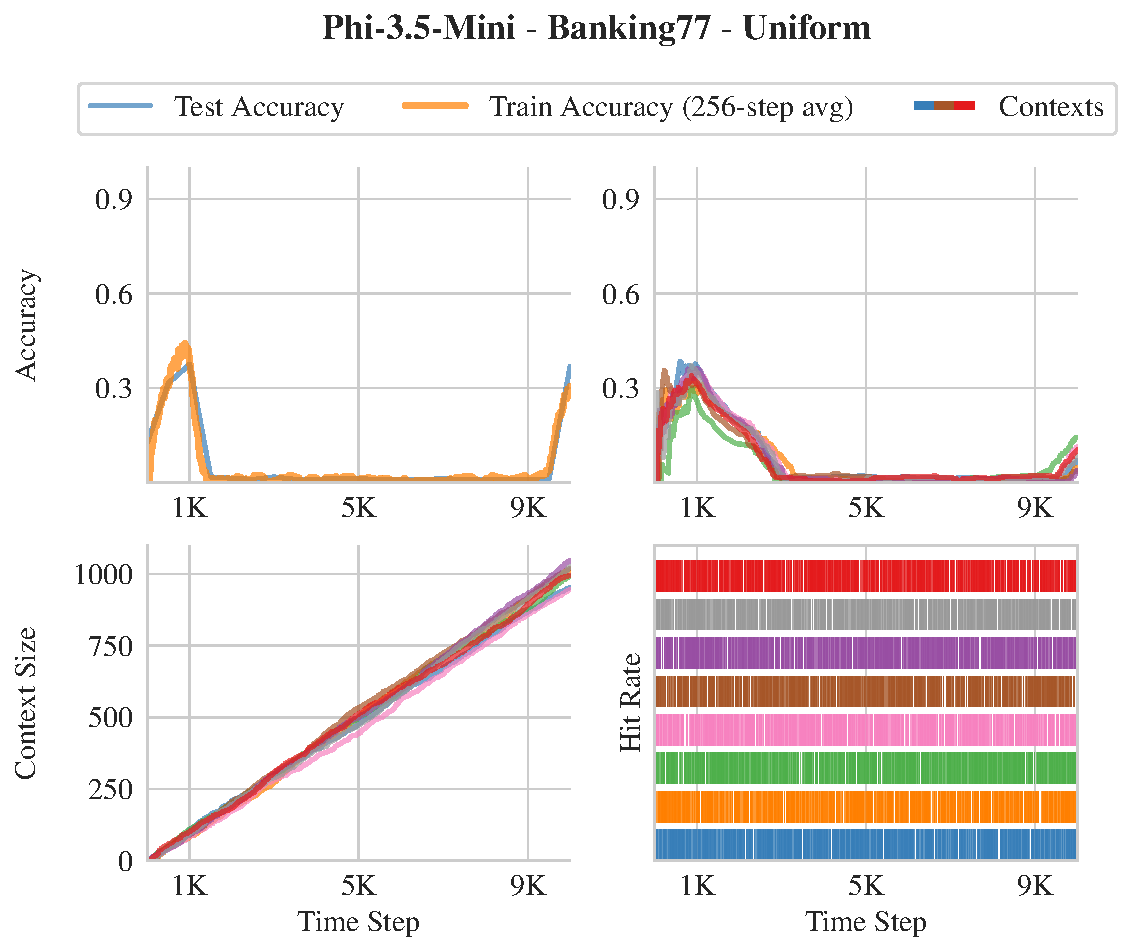
\includegraphics[width=0.6\textwidth]{figures/approximate_detailed_results/microsoft_Phi-3.5-mini-instruct_banking77_uniform.pdf}
\caption{\textbf{Detailed visualization of \appshort for \phillm, \banking with uniform context sampling.} We report test accuracy (top left), a 256-step running average of the training accuracy (bottom left), the training accuracy of each context (top right), and the hit rate of each context (bottom right).}
\end{figure}
\begin{figure}[htbp]
\centering
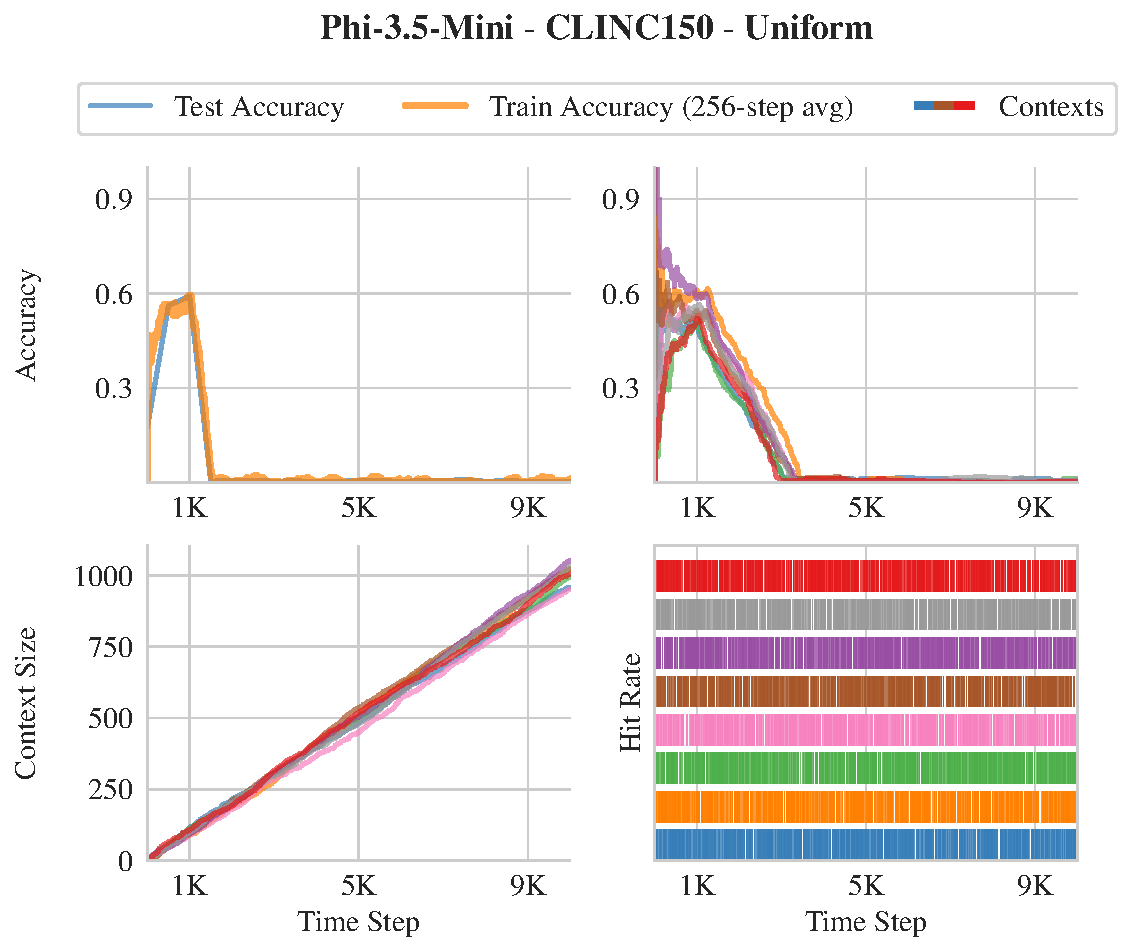
\includegraphics[width=0.6\textwidth]{figures/approximate_detailed_results/microsoft_Phi-3.5-mini-instruct_clinic150_uniform.pdf}
\caption{\textbf{Detailed visualization of \appshort for \phillm, \clinic with uniform context sampling.} We report test accuracy (top left), a 256-step running average of the training accuracy (bottom left), the training accuracy of each context (top right), and the hit rate of each context (bottom right).}
\end{figure}
